\documentclass[17pt,xcolor=table]{beamer} 
\definecolor{sbhs}{RGB}{255,69,50}
\definecolor{sbhs1}{RGB}{255,97,73}
\setbeamercolor{structure}{fg=sbhs}
\setbeamercolor{alerted text}{fg=sbhs1}
\usepackage{verbatim}
\usepackage{bm}
%\usepackage{txfonts}
\newenvironment{colorverbatim}[1][]
{
\color{blue}
}
{
\endverbatim
}
\usepackage{beamerthemesplit}
\usepackage{graphicx}
\usepackage{eso-pic}
\usepackage{beamerthemeshadow}
\beamertemplateshadingbackground{blue!5}{yellow!10}
\usepackage{beamerthemesplit}
\logo{
\includegraphics[height=1cm]{3t-logo.pdf}}
\begin{document}
\sffamily \bfseries
\title
[\scriptsize {Arduino access- IDE, Scilab \& Xcos}
\hspace{0.05cm}]
{\large{Performing LED blinking experiment on Arduino using Arduino IDE, Scilab and Xcos}}
\author [Manas R. Das]
{\small Talk To a Teacher \\http://sakshat.ac.in \\ National Mission on Education
  through ICT \\ http://spoken-tutorial.org \\ [0.2cm]
  Manas R. Das \\IIT Bombay \\ [0.1cm]
{\small 2 July 2015}}
\date{}
\begin{frame}
   \titlepage
\end{frame}

\begin{frame}[fragile]
\frametitle{Objectives}
In this tutorial we will learn to:
\begin{itemize}[<+-|alert@+>]
\item Connect Arduino to computer
\item Perform LED blinking experiment using Arduino IDE
\item Load scilab-arduino toolbox in scilab
\item Perform LED blinking experiment using scilab script
\item Perform LED blinking experiment using Xcos

\end{itemize}
\end{frame}

\begin{frame}
\frametitle{Software requirements}
\begin{itemize}[<+-|alert@+>]
\item Scilab 5.5.2 must be installed on your computer
\item I am using Windows-8 64 bit OS
\end{itemize}
\end{frame}

\begin{frame}
\frametitle{Scilab}
\begin{itemize}[<+-|alert@+>]
\item Download scilab from \\{\color{red} www.scilab.org}
\item Watch Scilab installation spoken tutorial available at {\color{red} spoken-tutorial.org}
\end{itemize}
\end{frame}



\begin{frame}[fragile]
\frametitle{Prerequisites}
\begin{itemize}[<+-|alert@+>]
\item Need of Origin folder
\item Save it on desktop
\end{itemize}

\end{frame}


\begin{frame}[fragile]
\frametitle{Arduino with shield}
\begin{figure}
\centering
\begin{minipage}{0.45\textwidth}
\centering
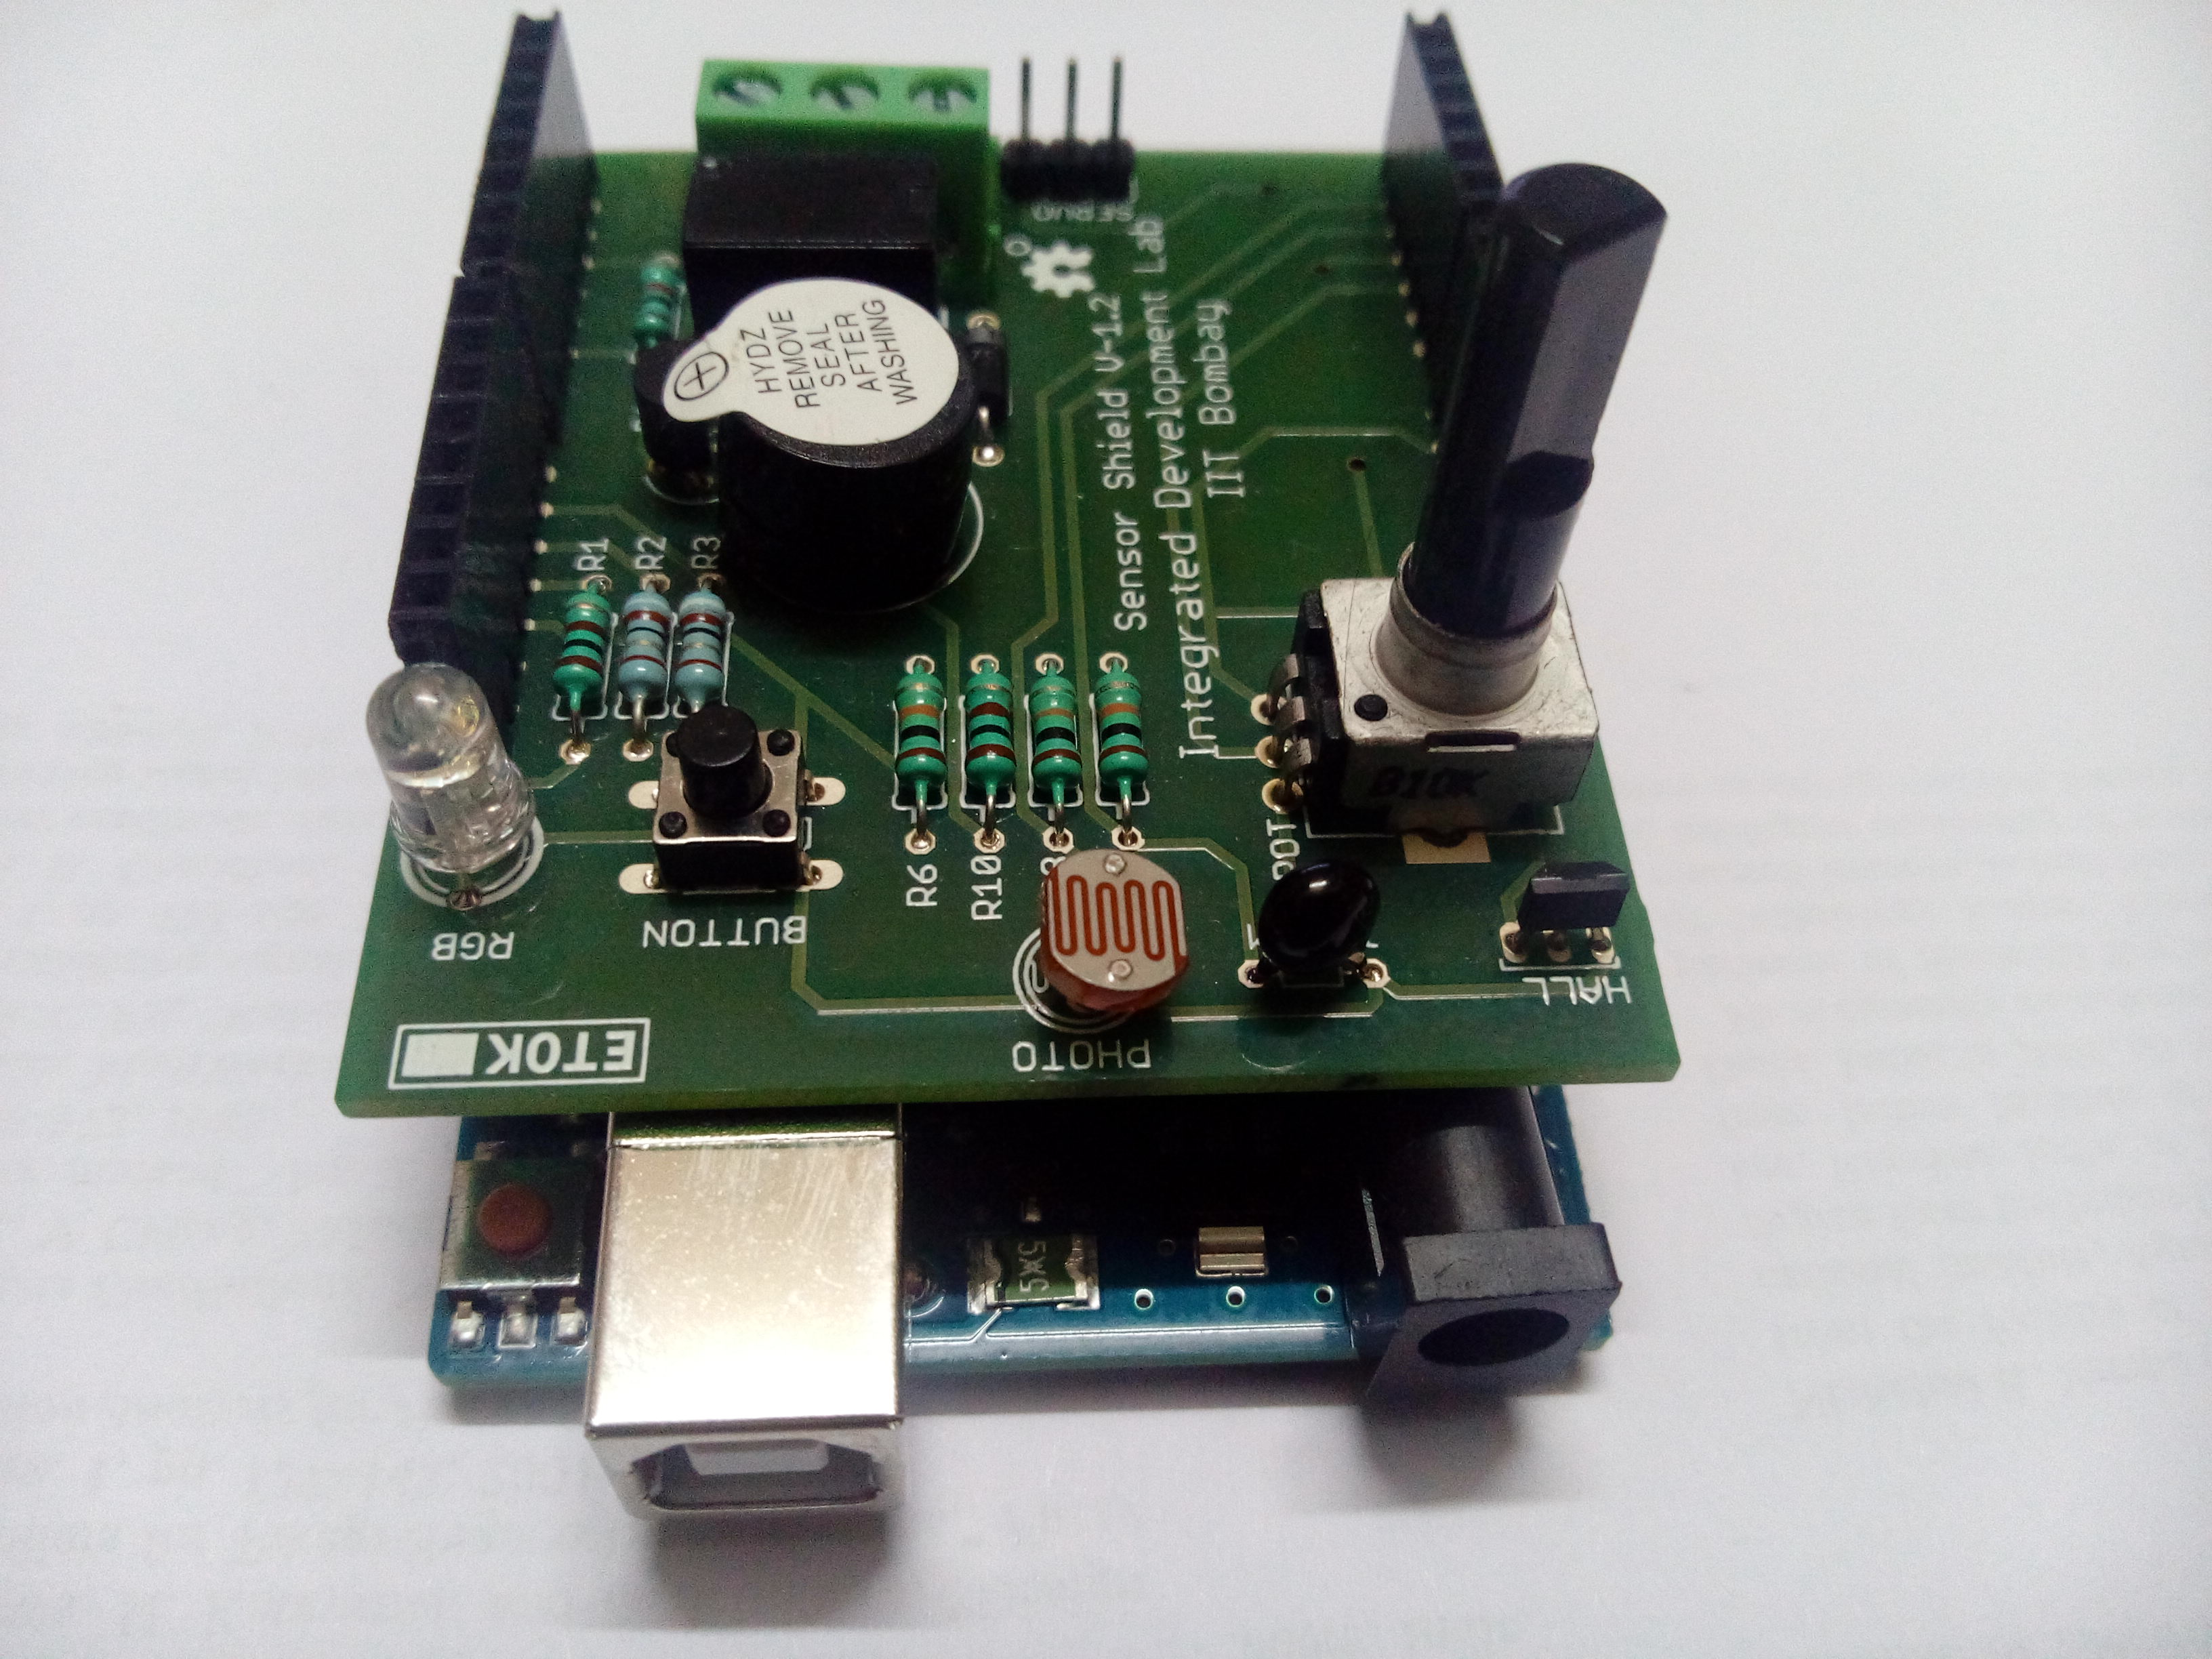
\includegraphics[width=1\linewidth]{arduino-shield-top.jpg}
\end{minipage}
\begin{minipage}{0.45\textwidth}
\centering
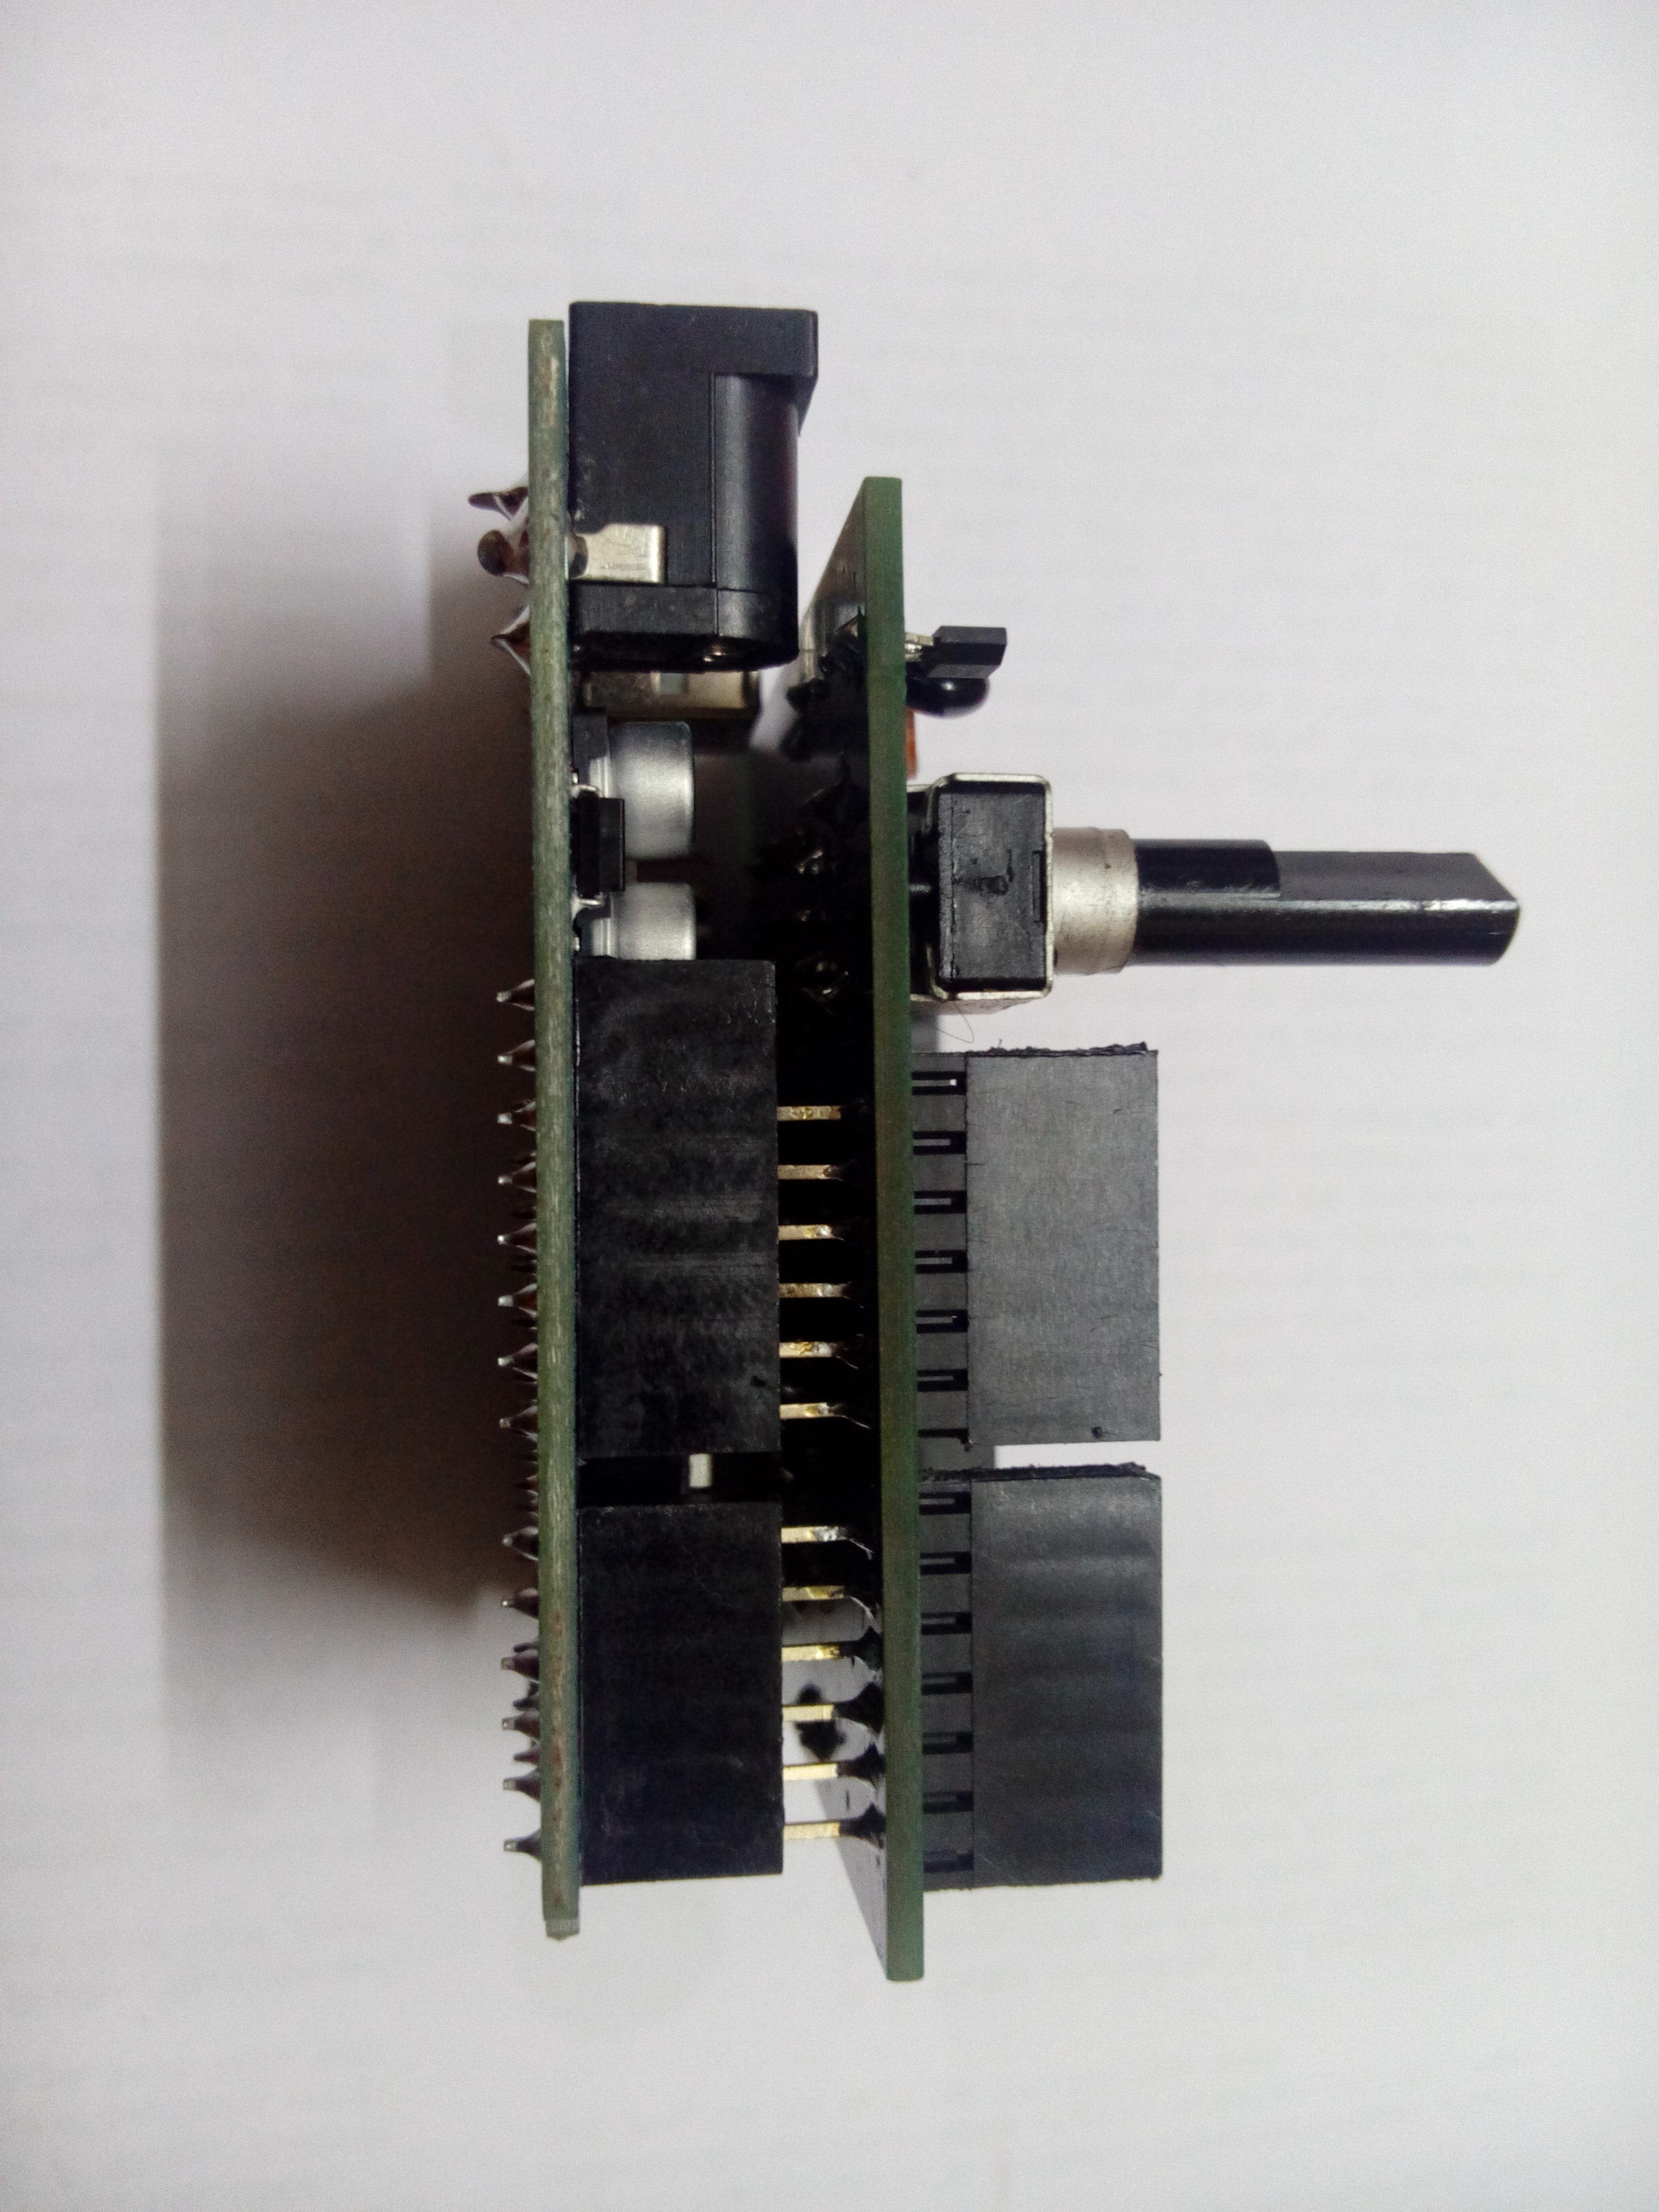
\includegraphics[width=0.9\linewidth, angle=90]{arduino-shield-side.jpg}
\end{minipage}
\end{figure}
\end{frame}


\begin{frame}[fragile]
\frametitle{Scilab-Arduino toolbox}
\begin{itemize}[<+-|alert@+>]
\item Scilab by default cannot communicate with arduino
\item Functionality provided using scilab-arduino toolbox
\item Toolbox available for both windows and linux
\end{itemize}

\end{frame}

\begin{frame}[fragile]
\frametitle{Scilab-Arduino toolbox Contd...}
\begin{itemize}[<+-|alert@+>]
\item Toolbox located at Origin/tool/windows or Origin/tools/linux
\item Requires a dedicated firmware to work with arduino
\item Firmware located at Origin/tools/arduino-firmware
\end{itemize}

\end{frame}
 
\begin{frame}[fragile]
\frametitle{Summary}
In this tutorial, we have learnt how to,
\begin{itemize}[<+-|alert@+>]
\item Perform Arduino IDE installation
\item Perform LED blinking experiment using Arduino IDE
\item Load scilab-arduino toolbox in scilab
\item Perform LED blinking experiment using scilab script
\item Perform LED blinking experiment using Xcos
\end{itemize}
\end{frame}

\begin{frame}
\frametitle{About the Spoken Tutorial Project}
\begin{itemize}
\item Watch the video available at {\color{red} http://spoken-tutorial.org /What\_is\_a\_Spoken\_Tutorial}
\item It summarises the Spoken Tutorial project 
\item If you do not have good bandwidth, you can download and watch it
\end{itemize}
\end{frame}

\begin{frame}
\frametitle{Spoken Tutorial Workshops}The Spoken Tutorial Project Team 
\begin{itemize}
\item Conducts workshops using spoken tutorials
\item Gives certificates to those who pass an online test
\end{itemize}
For more details, contact \\ {\color{red}contact@spoken-tutorial.org}

\end{frame}

\begin{frame}
\frametitle{Acknowledgements}
\begin{itemize}
\item Spoken Tutorial Project is a part of the Talk to a Teacher  project
\item It is supported by the National Mission on Education through  ICT, MHRD, Government of India
\item More information on this Mission is available at: \\ {\color{red} http://spoken-tutorial.org \\ /NMEICT-Intro}
\end{itemize}
\end{frame}



\end{document}
